\chapter{Evaluation}
\label{chap:evaluation}
Biohadoops purpose is to facilitate the implementation of parallel algorithms on Hadoop. It is expected that the execution time of an algorithm reduces if it is parallelized (assuming the algorithm is suitable for parallelization). This chapter is devoted to the study of Biohadoops speedup characteristics and possible influencing factors.

Two bio-inspired optimization algorithms are used as benchmarks. Both use Biohadoop and its task system to solve a test problem. The algorithms are executed on a Hadoop cluster to study the impact on their execution times by varying problem sizes and number of workers.

The rest of this chapter is structured as follows: section \ref{chap:evaluation:cluster} provides information about the cluster used for the benchmarks. Section \ref{chap:evaluation:testproblems} describes the benchmarked test problems. Section \ref{chap:evaluation:benchmark-details} provides guidance  for the interpretation of the benchmark results. Finally, section \ref{chap:evaluation:result} presents the results, section \ref{chap:evaluation:discussion} gives a discussion about factors that influence the benchmarks.

\section{Cluster Hardware}
\label{chap:evaluation:cluster}
All experiments were performed on a Hadoop cluster with 6 identical computers. Each machine has the following specifications:

\begin{itemize}
  \item Intel Core2 Duo CPU E8200 @ \unit[2.66]{GHz} (2$\times$\unit[2.66]{GHz}, no hyperthreading)
  \item \unit[6]{MB} shared L2 cache, \unit[32]{KB} L1 data cache, \unit[32]{KB} L1 instruction cache
  \item \unit[4]{GB} (2$\times$\unit[2]{GB}) DDR2 RAM @ \unit[667]{MHz}
\end{itemize}

The computers are directly connected to the same Switch through a 1Gb (Gigabit) Ethernet network.

\section{Test Problems}
\label{chap:evaluation:testproblems}
Both implemented algorithms are part of the GA family. They differ in the number of objectives that they can handle. While NSGA-II is used to solve the MOP in section \ref{chap:evaluation:zdt3}, a simple GA is used to solve the SOP in section \ref{chap:evaluation:tiledmul}.

\subsection{ZDT-3}
\label{chap:evaluation:zdt3}
The first optimization algorithm is NSGA-II, used to find optimal solutions for the Zitzler–Deb–Thiele's function nr. 3 \cite{zitzler2000comparison}. ZDT-3 is part of the well known ZDT family of MOP. It was chosen because of its discontinuous optimal Pareto Front (see figure \ref{fig:zdt3}) that not every optimization algorithm can handle, e.g., gradient based algorithms. The expected outcome is to find an approximation to the optimal Pareto Front.

\begin{figure}
  \centering
  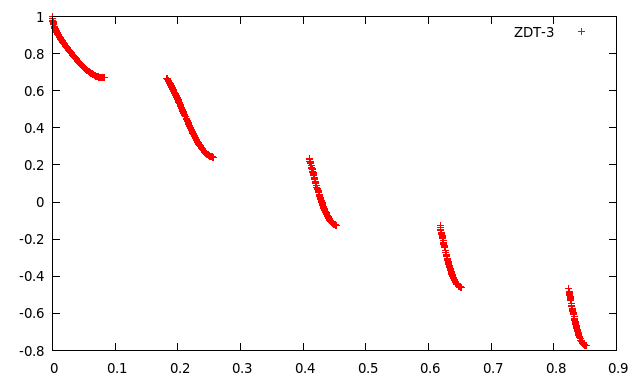
\includegraphics[width=110mm,natwidth=640,natheight=384]{zdt3.png}
  \caption[Optimal Pareto Front for ZDT-3]{Optimal Pareto Front for ZDT-3}
  \label{fig:zdt3}
\end{figure}

The ZDT-3 benchmarks are executed with genome sizes of 10, 100, 1000 and 10000. The genome size corresponds to the number of values of an individual and the dimension of the solution space. Each individual is represented by its genome. ZDT-3 can handle any genome size. Changing this number influences two properties of the ZDT-3 benchmark. First, increasing the number of genomes also increases the computation effort for the workers that generate new offsprings and compute their fitness. This is due to the fact that workers generate new individuals using parent genomes and that the ZDT-3 algorithm, used for the fitness computation, loops over all genomes. Second, the genome size influences the amount of data that has to be transferred between the master and the workers. Each worker repeatedly receives two parent individuals and returns an offspring and its computed fitness. The amount of data sent between master and workers is, therefore, related to the gnome size of each individual.

The implementation uses Biohadoop workers to create and evaluate the offsprings. Simulated Binary Crossover (SBX) and Parameter based mutation \cite{deb2000efficient} are used for the offspring creation. The fitness is computed using the ZDT-3 function. The selection of the fittest individuals for the next population is based on ranking and crowding distance and is performed on the master.

\subsection{Tiled Matrix Multiplication}
\label{chap:evaluation:tiledmul}
The second benchmark implements a GA to solve the SOP for finding optimal tile sizes for the tiled matrix multiplication (TMM). The objective is to minimize the execution time for a matrix multiplication. The expected outcome is a parameter set that minimizes the TMM execution time.

A matrix multiplication can be performed in different ways. The most obvious one is the standard algorithm:
\begin{lstlisting}
for i = 1 to n
  for j = 1 to m
    for k = 1 to l
      C(i,j) = C(i,j) + A(i,k) * B(k,j)
\end{lstlisting}

The matrix multiplication can be improved by loop tiling \cite{wolfe1989more}. The computation is performed on smaller blocks (tiles) of the matrices:
\begin{lstlisting}
for i0 = 1 to n, step blocksize_i
  for j0 = 1 to m, step blocksize_j
    for k0 = 1 to l, step blocksize_k
      for i = i0 to min(i0 + blocksize_i, n)
        for j = j0 to min(j0 + blocksize_j, m)
          for k = k0 to min(k0 + blocksize_k, l)
            C(i,j) = C(i,j) + A(i,k) * B(k,j)
\end{lstlisting}

If the blocks are small enough they fit into the L1 CPU cache which results in a speedup. For example, the average of ten consecutive test multiplications of two matrices of size 1024$\times$1024 took 11.384 seconds for the simple matrix multiplication. It took 2.669 seconds for the tiled multiplication with tile sizes $i=32$, $j=32$ and $k=32$. Both tests were performed on a single computer of the cluster. This numbers show that it is appropriate to use the tiled approach for the matrix multiplication. But the speed of TMM depends heavily on the tile sizes, the same tiled multiplication as above with tile sizes of $i=1$, $j=1$ and $k=1$ took 25.683 seconds to finish, an increase of about 10 times compared to a good tile size. Because of the number of possible tile size combinations and the time it takes to execute a matrix multiplication (e.g. matrix size=1024, 2 seconds for a matrix multiplication: $1024^3 \times 2 = 2\times{10^9} $ seconds), it is not feasible to do an exhaustive search for the optimal tile sizes.

An optimization algorithm can be used to find the (near) optimal tile sizes for the different loops. In this case, the optimization is done using a GA. The implementation uses Biohadoops workers to create and evaluate an offspring. For the offspring creation, Simulated Binary Crossover (SBX) and Parameter based mutation are used. The fitness is computed as the time it takes to multiply two matrices using a given tile size. The selection of the fittest individuals for the next population is performed on the master.

The TMM benchmarks are executed with matrix sizes of 128$\times$128 and 256$\times$256. The matrix size influences the number of computations that need to be performed for a full matrix multiplication and, therefore, also influences the execution time. In contrast to ZDT-3, the matrix size has no impact on the amount of data transferred between the master and the workers. The matrices are part of the ``initial data'' (see chapter \ref{chap:impl:worker}) and, hence, transferred exactly once to every worker. The task data consists of two parent individuals that are transferred from the master to the workers to create a new offspring and compute its fitness. The data transferred from a worker to the master contains the offspring and its computed fitness value. Each individual consists of its tile sizes for $i$, $j$ and $k$.

\section{Benchmarks and Results}
\label{chap:evaluation:benchmark-results}
This section is devoted to the examination of the benchmark results. First, the execution times of standalone, single threaded, sequential versions of the test problems are evaluated. Each of this standalone benchmarks is repeated five times to improve the reliability of the results. The informations gathered are used to calculate the lower and upper boundaries of achievable speedups for parallel Biohadoop versions. Then, the true Biohadoop benchmark speedups are calculated based on the mean run times of the according sequential versions. The reason to use mean execution times is that the sequential execution times used for the speedup boundary computations are not automatically the 

The correctness of the benchmark outputs is checked at the end of this section.

\subsection{Standalone Sequential Benchmarks}
Standalone, single threaded, sequential versions of the test problems from section \ref{chap:evaluation:testproblems} are used to compute the maximum speedups achievable through parallelization. Their execution times are also the basis for the speedup calculations of the parallelized Biohadoop versions of test problems.

The standalone implementations are written in Java. They are executed on a single machine of the cluster, run without Biohadoop and its task system and perform no network communication at all. The same parameters as for Biohadoop benchmarks are used, with one exception: the number of workers is not taken into account, since the implementations are sequential and single threaded.

Table \ref{table:sequential-runtimes} shows the maximum and minimum sequential execution times for the test problems, together with their mean values. The mean values are used further on to calculate the maximum achievable speedups and the speedups achieved when Biohadoop is used for parallelization.

Usage of mean values hides some of the complexity of speedup calculations at the price of precision. An exact solution would compute the theoretical speedups based on the code and its execution. This approach must take into account the program instructions, the machine architecture, cache usage and many other factors. It would be beyond the scope of this thesis to compute such a maximum theoretical speedup.

Another approach is to compute the lower and upper speedup boundaries based on the best and worst serial-to-parallel run time ratios measured. The approach was not persecuted for three reasons:
\begin{itemize}
  \item The lower and upper bounds are not absolute and it is highly probable that they change with additional measurements. So lower and upper bounds are, like the mean values, only approximations and it must be considered that the results may vary with additional benchmarks.
  \item The sequential run times used for the speedup boundary computations are not automatically the best choices to compute the speedups for parallel versions. Consider a sequential version that has very good serial-to-parallel ratio (low serial part, large parallel part) but a very long runtime. It would be used to compute a speedup boundary, probably the upper one. But it is not a good idea to use it for the computation of parallel speedup, as it may deliver results that don't reflect the general case.
  \item The complexity increases and 
\end{itemize}

Therefore, the mean values are used from here on for the speedup calculations.

\begin{table}
  \centering
  \caption{Execution times for standalone sequential implementations}
  \begin{tabular}{lrrr}\toprule[2pt]
    Test Problem &  Min. [s] & Max. [s] & Mean [s] \\ \midrule
    NSGA-II, 10 genomes & 2.852 & 3.049 & 2.907 \\
    NSGA-II, 100 genomes & 2.956 & 3.242 & 3.0463 \\
    NSGA-II, 1000 genomes & 7.673 & 8.865 & 8.497 \\
    NSGA-II, 10000 genomes & 71.390 & 72.150 & 71.792 \\
    128$\times$128 tiled mul & 132.066 & 178.639 & 153.968 \\
    256$\times$256 tiled mul & 1500.705 & 1587.130 & 1548.717 \\ \bottomrule[2pt]
  \end{tabular}
  \label{table:sequential-runtimes}
\end{table}


% The achievable speedup is computed as the mean value of five repetitions.
For the computation of maximum achievable speedups, the formula $S = T / (T - t_p)$ of Amdahl's law \cite{amdahl1967validity} is used. $S$ is the achievable speedup, $T$ is the execution time of the sequential algorithm and $t_p$ is the time spent in code parts that can be parallelized. The parallel code parts consist of offspring creation and evaluation. Workers execute the parallel code parts when the test problems are executed with Biohadoop.

The maximum achievable speedups in table \ref{table:speedup_bounds} show that the ZDT-3 benchmark is not well-suited for parallelization. This is due to the fact that the calculation of the ZDT-3 function is not compute intense. The sequential part of NSGA-II has a large influence on the whole algorithm runtime. This may be different for a more compute intense objective function. The TMM speedup bounds instead show that TMM is a good candidate for parallelization.


\begin{table}
  \centering
  \caption{Upper and lower speedup bounds}
  \begin{tabular}{lrrr}\toprule[2pt]
    Test Problem & Lower bound & Upper bound & average \\ \midrule
    NSGA-II, 10 genomes & 11.923 & 12.568 & 12.149 \\
    NSGA-II, 100 genomes & 8.025 & 9.640 & 8.978 \\
    NSGA-II, 1000 genomes & 10.103 & 11.774 & 11.281 \\
    NSGA-II, 10000 genomes & 11.330 & 11.955 & 11.586 \\
    128$\times$128 tiled mul & 178.341 & 241.770  & 206.729 \\
    256$\times$256 tiled mul & 248.950  & 280.542 & 265.073 \\ \bottomrule[2pt]
  \end{tabular}
  \label{table:speedup_bounds}
\end{table}

The execution time of a benchmark is composed of the time Biohadoop needs to start up and the algorithm execution time (see figure \ref{fig:execution-times}). The start up begins with Biohadoops submission to Hadoop and ends when the algorithms \texttt{run} method is invoked. The algorithm execution time starts with the invocation of the algorithms \texttt{run} method and ends when this method returns.

\begin{figure}
  \centering
  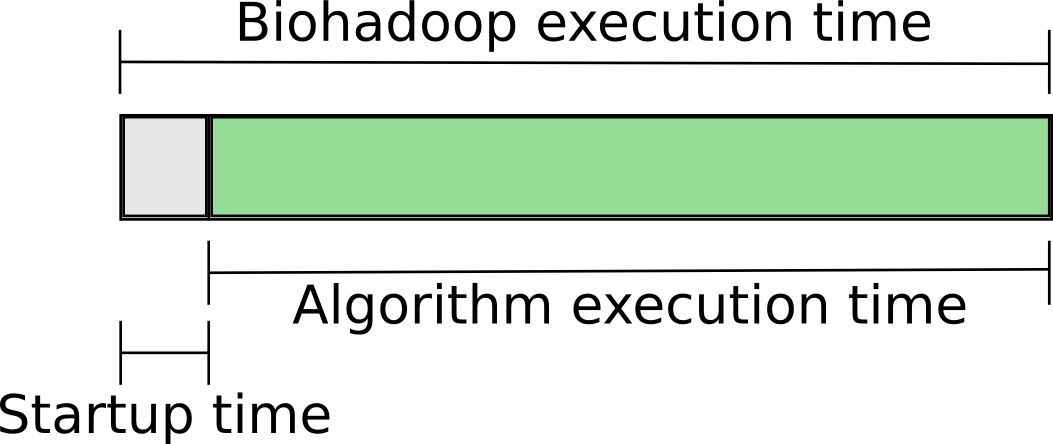
\includegraphics[width=60mm,natwidth=1053,natheight=444]{execution-times.png}
  \caption[Division of Biohadoop execution times]{Biohadoop execution times are composed of start up times and algorithm execution times}
  \label{fig:execution-times}
\end{figure}

The distinction between start up time and algorithm execution time is made because the main part of the start up time is spent between the application submission to YARN and the beginning of its execution. It is not possible to predict when an application is executed by Hadoop as it depends on different factors like the available cluster resources. To minimize the impact of this uncertainty, the benchmark measurements are based on the algorithm execution time, without the application start up time.

% The start up time over all benchmarks range from \unit[2.378]{s} to \unit[6.147]{s}, with a median of \unit[3.864]{s}, a \unit[25]{\%} quartile of \unit[3.145]{s} and a \unit[75]{\%} quartile of \unit[4.258]{s}. The mean value is \unit[3.781]{s}. These start up times are close to each other, because the used cluster was completely dedicated to the benchmarks. The start up may take longer when the cluster usage is higher.

\section{Results}
\label{chap:evaluation:result}
This section is devoted to the examination of the benchmark results. First, the execution times of standalone sequential versions of the test problems are evaluated. This information is used to calculate speedup boundaries for the parallel Biohadoop versions. Then, the Biohadoop benchmark speedups are calculated based on this numbers. The correctness of the benchmark outputs are checked at the end of this section.



% The algorithm execution time results for the benchmarks can be found in the boxplots in figures \ref{fig:nsga_250_100_10} to \ref{fig:nsga_250_100_10000} for the ZDT-3 benchmarks and in figures \ref{fig:tiledmul_250_100_128x128} and \ref{fig:tiledmul_250_100_256x256} for the TMM. The number of workers and the algorithm execution time is plotted on the x-axis and y-axis, respectively.

\subsection{Biohadoop Benchmark Speedups}
The benchmarks are executed on the cluster described in section \ref{chap:evaluation:cluster}. The assumption is that the execution time of an algorithm depends both on the problem size and the number of workers. To evaluate this assumption, the algorithms presented in section \ref{chap:evaluation:testproblems} are executed with different problem sizes and different numbers of workers. For NSGA-II the problem size is defined as the genome size, for TMM it is the matrix size. The number of workers range for both test problems from 1 to 15.

All performed benchmarks have the following settings in common:
\begin{itemize}
  \item The number of iterations is set to 250.
  \item The population size is set to 100.
  \item The distribution index $n_c$ for the SBX crossover is set to 20.
  \item The distribution index $n_m$ for the mutation is set to 20.
  \item The mutation probability for each offspring value is set to $1/n$, i.e., on average one offspring value is mutated.
\end{itemize}

Each benchmark is repeated five times to improve the reliability of the results, making it 300 benchmark runs for ZDT-3 (4 genome sizes $\times$ 15 worker setting $\times$ 5 repetitions) and 150 benchmark runs for TMM (2 tile sizes $\times$ 15 worker settings $\times$ 5 repetitions).




The algorithm execution times using the Biohadoop version of the benchmarks of the benchmarks are measured and used to calculate the speedups for the benchmarks using the formula $S = T_S / T_P$. Here, $S$ is the speedup. The sequential time $T_S$ is taken from the standalone sequential versions of the benchmarks. $T_P$ is the time for the execution with 1 to 15 parallel workers.

Figure \ref{fig:speedup} depicts the speedups for all test problems with respect to increasing worker sizes. The ZDT-3 benchmarks show poor results. This is not surprising as the maximum theoretical speedups of this problem are small (see table \ref{table:theoretical_speedup}) and the communication overhead is bigger compared to TMM. The only unexpected outcome was that the benchmarks scale very bad with a maximum speedup of 2.498 for 1000 genomes. The reason is that the ZDT-3 benchmarks are CPU bound by the master, as the investigations in section \ref{chap:evaluation:result:zdt3} suggest.

TMM demonstrate better results, the maximum speedup was 10.507 for a matrix size of 128$\times$128. In this case, the speedup grows near linear or even slightly better than linear with the number of workers. That a speedup is better than linear is usually suspicious but can be explained by the fact that each benchmark was repeated five times and the average times of this five executions were taken to compute the speedups. Five executions seem to be too small for getting smooth results, especially when taking into account that the YARN container placement has big influences on the execution times.

The speedups for the 128$\times$128 TMM increase until a worker size of 12 is reached. At this point, no more improvements are achieved. The reason for this is the limited number of CPUs in the cluster.

The speedup for the 256$\times$256 TMM benchmark is worse compared to the 128$\times$128 TMM, although it also grows nearly linear until 12 workers.

\begin{figure}
  \centering
  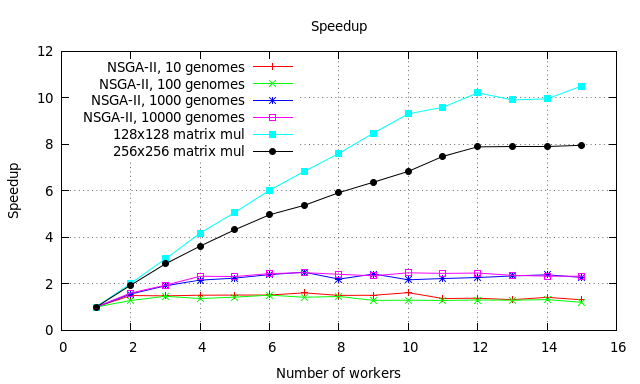
\includegraphics[width=130mm,natwidth=640,natheight=384]{speedup.png}
  \caption[Speedups for ZDT-3 and TMMs]{Speedups for ZDT-3 and TMMs}
  \label{fig:speedup}
\end{figure}

\subsection{Comparison with Implementation without Hadoop}




% \begin{itemize}
%   \item Free resources (CPU, RAM, Network) on the machine: The utilization of a machine by other processes influences the execution times.
%   \item Network package size: The network in use has a maximum package size. If data packets exceed this size, they need to be chunked into several smaller packets.
%   \item JIT (Just-in-time compiler): the Java just-in-time compiler compiles Java byte code into machine executable code that can be executed faster. This compilation is done only if a a certain part of a Java program is called several times (typically after 10000 calls). JIT optimized code executes faster than interpreted code, but takes itself some time to get compiled
%   \item Netty and Kryo performance: Netty provides the network functionality for Biohadoop, Kryo is used for serialization. Both are executed on the master and worker processes and have influence on the algorithm execution times due their need for resources. It is hard to estimate how Netty and Kryo behave for different data sizes, e.g., kt is tunable how much buffer memory Kryo allocates by default for serialization/deserialization. 
%   \item L1 / L2 cache sharing and pollution: The CPUs used for the benchmarks have a per-core L1 cache of \unit[32]{KB} and a shared L2 cache of \unit[6]{MB}. Since several processes run on each machine (.e.g. the operating system and the Hadoop processes), it is hard to estimate how much cache is available for the benchmark execution.
%   \item YARN container placement: The benchmark algorithm execution times depend on the placement of the YARN containers.
%   \item YARN container startup time (master and worker containers): It may take arbitrary time for YARN to start a container. This can not be influenced.
%   \item Operating System (OS): The OS needs resources itself. It provides the resources for the benchmark execution and the transmission of network data. Especially the second component can have an influence on the execution times.
% \end{itemize}

% Table \ref{table:theoretical_speedup} gives an impression how well the benchmark problems are suited to parallelization by showing the maximum theoretical speedup. The theoretical speedup was calculated using the formula $S = T / (T - t_p)$ from Amdahl's law \cite{amdahl1967validity}, where $S$ is the speedup, $T$ the algorithm execution time and $t_p$ is the time spent in code parts that are parallelized using Biohadoops task system. $T$ and $t_p$ were taken from the average benchmark times with one worker.

% \begin{table}
%   \centering
%   \caption{Theoretical speedups}
%   \begin{tabular}{lr}\toprule[2pt]
%     Test Problem & Theoretical Speedup \\ \midrule
%     NSGA-II, 10 genomes & 7.028 \\
%     NSGA-II, 100 genomes & 7.600 \\
%     NSGA-II, 1000 genomes & 12.008 \\
%     NSGA-II, 10000 genomes & 11.124 \\
%     128$\times$128 tiled mul & 81.359 \\
%     256$\times$256 tiled mul & 212.169 \\ \bottomrule[2pt]
%   \end{tabular}
%   \label{table:theoretical_speedup}
% \end{table}

% One can see from the theoretical speedups that ZDT-3 is not well suited for parallelization. This is due to the fact that the fitness evaluation is not compute intense. Its time consuming part is a sum over the genomes of an individual, implemented as loop. For example, in the case of 10 genomes per individual this loop would be repeated 10 times. Bigger genome sizes mitigate this effect but have the drawback that the communication time between the master and the workers increases, which negatively affects the speedup. TMMs on the other side show a big potential for parallelization.

\section{Discussion}
\label{chap:evaluation:discussion}

\subsection{Influence of YARN Container Placement}
The first thing to note when looking at the figures \ref{fig:nsga_250_100_10} to \ref{fig:tiledmul_250_100_256x256} is that the five benchmark times for a given setting (e.g. NSGA-II, 10 genomes) and one worker are very different. The explanation for this effect can be found in the YARN container placement. If a worker container is executed on the same machine as the master container, they communicate without using the physical network. This effect brings a huge performance gain, as can be seen for example in figure \ref{fig:nsga_250_100_100}. In the single worker benchmarks, 4 out of 5 benchmarks executed with both the master and worker container running on the same machine. The result was a \unit[50]{\%} better performance (\unit[9.761]{s} average) compared to the fifth benchmark (\unit[14.164]{s}) where the master and worker were executed on different machines. Potential research projects could focus on a Hadoop scheduler that tries to put a YARN ApplicationMaster and its containers on the same machine to reliably produce similar results.

The number of worker containers running on the same machine as the master can also have a negative effect on the execution times. This is especially true if the master is already at the limit of the machines resources and must share them with the workers. An example for this can be found in figure \ref{fig:nsga_250_100_10} for 8 workers. Two worker containers were executed on the same machine as the master during 2 out of 5 benchmarks. The execution time results were \unit[87.977]{s} and \unit[88.014]{s}. In the remaining 3 benchmarks, only one worker container was executed on the same machine as the master, leaving more resources to the master. This results in execution times of \unit[68.423]{s} on average, a difference of more than \unit[20]{\%}.

Therefore, it depends on the available resources of a machine if the execution of worker containers on the same machine as the master container provides benefits or drawbacks. If a resource like CPU or network is already at its limit, additional worker containers slow the whole Biohadoop execution down. If there are enough resources available, the execution of worker containers on the same machine as the master provides benefits, as the communication between the master and the workers can be performed without network usage.

The location of the YARN containers can currently not be influenced, but discussions by the YARN developers suggest that future versions of YARN will support this feature.

% \subsection{CPU Influence}
% The CPU has big influence on the algorithm execution times. If the CPU u
% 
% \subsection{RAM Influence}
% All benchmarks start with \unit[256]{MB} of Java heap memory, which is enough for the containers to execute without causing excessive garbage collections. This was established by using the tool jvisualvm (delivered with Java) for the ZDT-3 benchmark with 10000 genomes and the TMM with a matrix size of 256x256. The memory usage for the master container is at about \unit[100]{MB} to \unit[150]{MB}. The activity of Java's garbage collector at the master takes about \unit[5]{\%} of the CPU time. This value would be significantly higher in case of a memory problem. The memory usage for a worker is even lower and lies in the range of \unit[5]{MB} to \unit[30]{MB}. Again, this numbers show no significant memory problems.

\subsection{ZDT-3}
\label{chap:evaluation:result:zdt3}
The next thing to notice are the speedups for the ZDT-3 benchmarks. ZDT-3 is not well suited for parallelization as can be seen from the speedups in table \ref{table:speedup_bounds}, but the results are even worse than expected, with maximum speedups of 1.619 for 10 genomes, 1.513 for 100 genomes, 2.498 for 1000 and 2.479 for 10000 genomes. Figure \ref{fig:speedup} shows the speedup results of the ZDT-3 benchmarks together with the speedups for TMM.

\begin{figure}
  \centering
  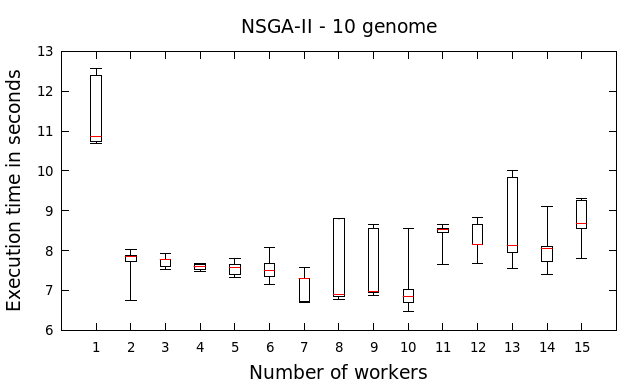
\includegraphics[width=100mm,natwidth=640,natheight=384]{nsgaii_250_100_10.png}
  \caption[ZDT-3 execution times for a genome size of 10]{ZDT-3 execution times for a genome size of 10}
  \label{fig:nsga_250_100_10}
\end{figure}
\begin{figure}
  \centering
  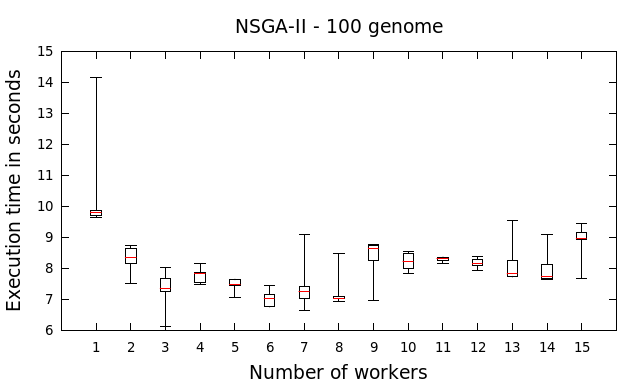
\includegraphics[width=100mm,natwidth=640,natheight=384]{nsgaii_250_100_100.png}
  \caption[ZDT-3 execution times for a genome size of 100]{ZDT-3 execution times for a genome size of 100}
  \label{fig:nsga_250_100_100}
\end{figure}
\begin{figure}
  \centering
  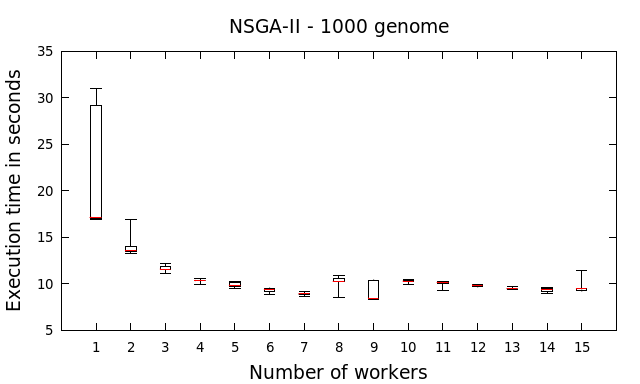
\includegraphics[width=100mm,natwidth=640,natheight=384]{nsgaii_250_100_1000.png}
  \caption[ZDT-3 execution times for a genome size of 1000]{ZDT-3 execution times for a genome size of 1000}
  \label{fig:nsga_250_100_1000}
\end{figure}
\begin{figure}
  \centering
  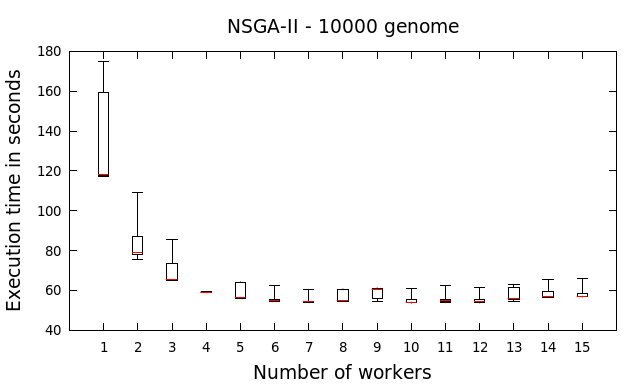
\includegraphics[width=100mm,natwidth=640,natheight=384]{nsgaii_250_100_10000.png}
  \caption[ZDT-3 execution times for a genome size of 10000]{ZDT-3 execution times for a genome size of 10000}
  \label{fig:nsga_250_100_10000}
\end{figure}

The ZDT-3 benchmarks seem to suffer from the lack of one or more resources (bound by the resources), which prohibits further speedup increases. The investigations show that the ZDT-3 benchmarks are not bound by memory, i.e., memory issues don't slow the execution down. All benchmarks start with \unit[256]{MB} of Java heap memory, which is enough for the containers to execute without causing excessive garbage collections. This was established by using the tool jvisualvm (delivered with Java) for the ZDT-3 benchmark with 10000 genomes. The memory usage for the master container is at about \unit[100]{MB} to \unit[150]{MB}. The activity of Java's garbage collector, a good indicator for memory problems, ranges from \unit[3]{\%} to \unit[5.5]{\%} of the CPU time, with an average of \unit[3.8]{\%}. The memory usage for a worker is even lower and lies in the range of \unit[5]{MB} to \unit[30]{MB}. This numbers show no significant memory problems.

The next step is to investigate the network performance. Calculations give a first hint to understand if the bad speedups can be explained with the saturation of the \unit[1]{Gb} network (a small ``b'' denotes bits, a big ``B'' denotes bytes, e.g., \unit[1]{Gb} = 1 gigabit, \unit[1]{GB} = 1 gigabyte). In each benchmark, 250 iterations on 100 individuals are performed, resulting in 25000 tasks. The tasks are send from the master to the workers and the workers return the results. The task data send from the master to the worker contains two individuals. Each individual consists of its genome, where each value in the genome is of type \texttt{double} (8 bytes). For a genome size of 10, this makes 2 (parents) $\times$ 10 (genomes) $\times$ 8 (bytes) $\times$ 25000 (tasks) = 4000000 bytes (\unit[4]{MB}) or \unit[32]{Mb} of data that needs to be transferred from the master to the workers during the benchmark. The size of the results sent from the workers to the master is about the half, as it consists of an individual (the offspring) and its fitness (the fitness is composed of two \texttt{double} values). This fact allows to use the outgoing data amount as upper bound for the network usage: if the outgoing data rate doesn't exceed the network bandwidth. This will be true also for the incoming data. Table \ref{table:network} shows the results for all genome sizes together with the best algorithm execution times. One can see from the table that the benchmark data can be transferred on the \unit[1]{Gb} Ethernet network during the according fastest algorithm execution time.

\begin{table}
  \centering
  \begin{tabular}{r|r|r|r}
    genomes & data [Mb] & \parbox[t]{3cm}{theoretical\\transfer time [s]} & \parbox[t]{3cm}{fastest algorithm\\execution time [s]}\\ \hline
    10 & 32 & 0.032 & 7.072 \\
    100 & 320 & 0.32 & 7.031 \\
    1000 & 3200 & 3.2 & 8.910 \\
    10000 & 32000 & 32 & 55.475 \\
  \end{tabular}
  \caption{Amount of network data sent from master to workers, theoretical transfer time and fastest algorithm execution}
  \label{table:network}
\end{table}

Additional experiments were performed to improve the confidence in the calculations and to establish the true achievable data rate for the network, given different message sizes. The experiments measure the peak network bandwidth using a small Java program and iftop.\footnote{\url{http://www.ex-parrot.com/pdw/iftop/} last access: 08.12.2014} The Java program uses the same communication techniques as Biohadoop (Netty + Kryo) and performs repeated request/response cycles between a master and several workers. The exchanged messages consist of 20, 200, 2000 or 20000 \texttt{double} values, corresponding to two parent individuals in the according ZDT-3 benchmarks. The resulting peak bandwidth was \unit[134]{Mb/s} for 20, \unit[489]{Mb/s} for 200, \unit[901]{Mb/s} for 2000 and \unit[552]{Mb/s} for 20000 \texttt{double} values. The CPU on the master was the limiting factor for 20, 200 and 20000 \texttt{double} values. For 2000 \texttt{double} values, the network was saturated at \unit[901]{Mb/s} and, therefore, the limiting factor. No studies were performed to explain why the experiments delivered the best results with 2000 values as this lies out of the scope of this thesis.

One phenomena regarding the network bandwidth needs further investigation. The above measurements show a peak data rate of \unit[552]{Mb/s} for the case of 20000 \texttt{double} values. If this data rate is taken as a basis for the ZDT-3 benchmark with 10000 genomes, one can calculate that more than \unit[55]{s} are needed to exchange \unit[32]{Gb} of data over the network between the master and its workers (\unit[32000]{Mb} / \unit[552]{Mb/s} = \unit[57.97]{s}). The explanation can be found once more in the YARN container placement. The \unit[552]{Mb/s} peak bandwidth is the data rate that is send through the Ethernet port to the cluster, but worker containers that run on the same machine as the master don't use this port for communication. Instead, they communicate through the local interface. iftop showed an additional combined data transfer rate of \unit[400]{Mb/s} (send and receive data rates are added) on the local interface when workers were running on the same machine as the master. This gives an aggregated peak data rate of \unit[700]{Mb/s} to \unit[800]{Mb/s} for the outgoing traffic, which is fast enough to transmit \unit[32]{Gb} of data in less than \unit[55]{s}. The execution times were higher in cases where no workers executed on the same machine as the master.

The calculations and additional experiments show that the network is fast enough to transfer the ZDT-3 benchmark data. The reason for the bad ZDT-3 speedups lie elsewhere.

This leads to the assumption that the benchmarks are CPU bound which was confirmed through observations of the CPU usage of the master. In the case of 10 and 100 genomes the CPU limit was reached by the master with two workers, for 1000 and 10000 genomes the limit was reached with four workers.

The high CPU utilization is caused by two effects: the first one is the object serialization/deserialization overhead that ranges between \unit[30]{\%} to \unit[40]{\%} for genome sizes of 10 and goes up to \unit[60]{\%} to \unit[70]{\%} for a genome size of 10000. Small genome sizes mean a high rate of both exchanged messages and serializations/deserializations. Large genome sizes reduce the rate of exchanged messages but increase the amount of work for a single serialization/deserialization.

The second effect is a direct consequence of computationally small worker tasks like in the case of 10 to 100 genomes: the master performs (beside the communication aspects) the algorithms for ranking and crowding distance. The workers return their results fast as the computation is not intense. Therefore, the master has to compute the ranking and crowding distance at short intervals. This results in a CPU utilization of about \unit[25]{\%} to \unit[30]{\%} only for this computations.

In conclusion, the ZDT-3 benchmarks are CPU bound by the master due to the small computational effort on the workers and the resulting fast exchange of many small messages. Increased genome sizes provide better speedup results, but are again limited by the CPU of the master, as they have higher demands for object serialization/deserialization. The performance of the \unit[1]{Gb} network and the available memory are sufficient to not slow down the ZDT-3 benchmarks.

\subsection{Tiled Matrix Multiplication}
The optimization goal of this benchmark was to find optimal tile sizes such that a matrix multiplication performs as fast as possible. The theoretical speedups for TMM promise better results (see table \ref{table:theoretical_speedup}) as matrix multiplications are compute intense and clearly dominate the algorithm execution time. Figure \ref{fig:tiledmul_250_100_128x128} and \ref{fig:tiledmul_250_100_256x256} show the execution times. One can see that the execution times decrease with the number of workers. This scales until 12 workers, after which the execution times remain constant or even increase slightly. The reason for this is that the cluster offers 12 CPU cores in total. When all cores are fully utilized, which happens with 12 workers, additional workers have to share CPU resources. This negatively impacts the execution times. So, TMM is CPU bound by the workers.

\begin{figure}
  \centering
  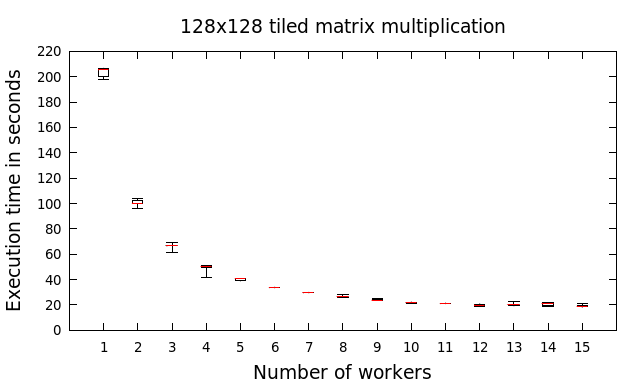
\includegraphics[width=100mm,natwidth=640,natheight=384]{tiledmul_250_100_128x128.png}
  \caption[TMM execution times for a matrix size of 128$\times$128]{TMM execution times for a matrix size of 128$\times$128}
  \label{fig:tiledmul_250_100_128x128}
\end{figure}
\begin{figure}
  \centering
  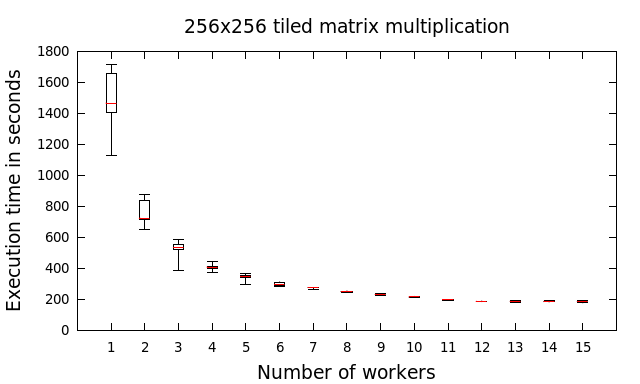
\includegraphics[width=100mm,natwidth=640,natheight=384]{tiledmul_250_100_256x256.png}
  \caption[TMM execution times for a matrix size of 256$\times$256]{TMM execution times for a matrix size of 256$\times$256}
  \label{fig:tiledmul_250_100_256x256}
\end{figure}

An additional advantage of TMM benchmarks over the ZDT-3 benchmarks is the small amount of data that needs to be transmitted. Like in the ZDT-3 benchmarks, each task data consists of two parents that are sent from the master to the worker, the result is an offspring with its fitness value. In contrast to ZDT-3 --- where an individual consists of a number of \texttt{double} values according to its genome size --- a TMM individual consists of the tile sizes for the $i$, $j$ and $k$ loop. Each of them is a single \texttt{integer} with 4 bytes. The total amount of data that needs to be transmitted from the master to the workers is therefore $2 \times 3 \times 4 \times 25000 = 600000$ bytes or \unit[4.8]{Mb}. Together with the computationally intense tasks of matrix multiplication on the workers (leading to lower network usage) and the absence of time consuming ranking and crowding distance algorithms on the master, this provides speedups of up to 10.507 for 128$\times$128 matrices and 7.961 for 256$\times$256 matrices.

The reason for the better performance of the 128$\times$128 benchmark over the 256$\times$256 benchmark is unknown. A possible explanation is that the tile sizes are taken from a bigger range (256 instead of 128) which makes it more likely that bad tile sizes are chosen. This is, however, pure speculation.


% \subsection{Speedups}
% Figure \ref{fig:speedup} depicts the speedups for all test problems with respect to increasing worker sizes. The ZDT-3 benchmarks show poor results. This is not surprising as the maximum theoretical speedups of this problem are small (see table \ref{table:theoretical_speedup}) and the communication overhead is bigger compared to TMM. The only unexpected outcome was that the benchmarks scale very bad with a maximum speedup of 2.498 for 1000 genomes. The reason is that the ZDT-3 benchmarks are CPU bound by the master, as the investigations in section \ref{chap:evaluation:result:zdt3} suggest.
% 
% TMM demonstrate better results, the maximum speedup was 10.507 for a matrix size of 128$\times$128. In this case, the speedup grows near linear or even slightly better than linear with the number of workers. That a speedup is better than linear is usually suspicious but can be explained by the fact that each benchmark was repeated five times and the average times of this five executions were taken to compute the speedups. Five executions seem to be too small for getting smooth results, especially when taking into account that the YARN container placement has big influences on the execution times.
% 
% The speedups for the 128$\times$128 TMM increase until a worker size of 12 is reached. At this point, no more improvements are achieved. The reason for this is the limited number of CPUs in the cluster.
% 
% The speedup for the 256$\times$256 TMM benchmark is worse compared to the 128$\times$128 TMM, although it also grows nearly linear until 12 workers.
% 
% \begin{figure}
%   \centering
%   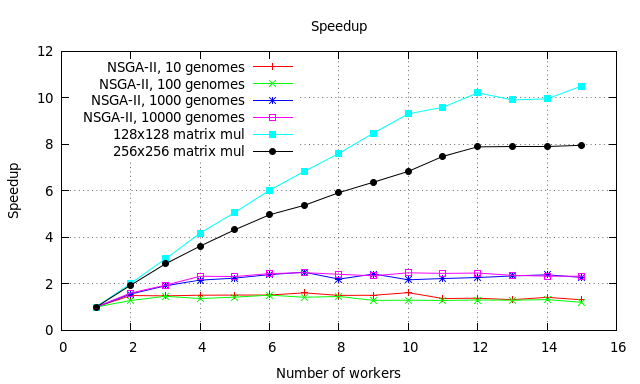
\includegraphics[width=130mm,natwidth=640,natheight=384]{speedup.png}
%   \caption[Speedups for ZDT-3 and TMMs]{Speedups for ZDT-3 and TMMs}
%   \label{fig:speedup}
% \end{figure}
